\begin{center}
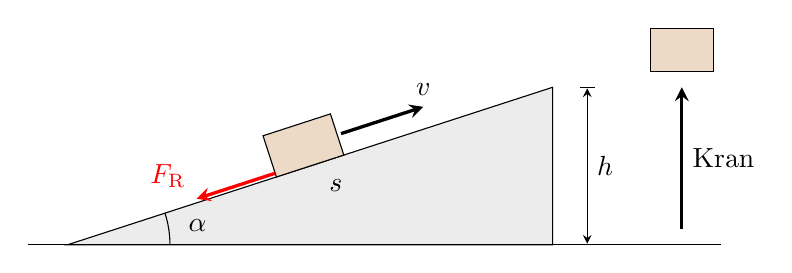
\begin{tikzpicture}[>=stealth]
 \draw[fill=gray!15] (0,0) -- (6.16,0) -- (6.16,2) -- cycle;
 \draw (-0.5,0) -- (8.3,0);
 \begin{scope}[shift={(3.08,1)}, rotate=18]
  \draw[fill=brown!30] (-0.45,0) rectangle (0.45,0.55);
  \draw[->, very thick] (0.5,0.27) -- (1.6,0.27) node[above] {$v$};
  \draw[->, very thick, red] (-0.45,0.05) -- (-1.5,0.05) node[above left] {$F_\mathrm{R}$};
 \end{scope}
 \draw (1.3,0) arc (0:18:1.3);
 \node at (1.65,0.25) {$\alpha$};
 \node[below right] at (3.2,0.95) {$s$};
 \draw[|<->|] (6.6,0) -- (6.6,2) node[midway, right] {$h$};
 \draw[fill=brown!30] (7.4,2.2) rectangle (8.2,2.75);
 \draw[->, very thick] (7.8,0.2) -- (7.8,2.0) node[midway, right] {Kran};
\end{tikzpicture}
\end{center}
Mit dem Kran (gleichmässiges Heben) ist nur die Hubarbeit nötig:
\begin{align}
 W_1 &= m\,g\,h
\end{align}
Auf der Rampe kommt die Reibungsarbeit dazu. Die Normalkraft ist $F_\mathrm{N} = m\,g\cos\alpha$, die Reibungskraft $F_\mathrm{R} = \mu\,m\,g\cos\alpha$ und der Weg $s = h/\sin\alpha$:
\begin{align}
 W_2 &= m\,g\,h + \mu\,m\,g\cos\alpha\cdot\frac{h}{\sin\alpha} = m\,g\,h\left(1+\frac{\mu}{\tan\alpha}\right)
\end{align}
Die Arbeit ist im zweiten Fall um den Anteil
\begin{align}
 \frac{W_2-W_1}{W_1} &= \relF \\
   &= \frac{\mur}{\tan\alrO} \\
   &= \rel \approx \result{\relP{0}{2}}
\end{align}
grösser. Masse und Höhe kürzen sich heraus.
